\documentclass{beamer}

\usepackage[brazilian]{babel}
\usepackage[utf8]{inputenc}
\usepackage{graphicx}
\usepackage{fontenc}
\usepackage{listings}
\usepackage{verbatim}
\usepackage{pxfonts}
\usepackage{graphicx}
\usetheme{Warsaw}

\title{Plugins no WordPress}
\subtitle{Fazendo o Negócio Direito}
\author{Vinicius Massuchetto}
\institute{Campus Party Brasil 2013}
\date{Fevereiro de 2013}

\lstset{%
  breakatwhitespace,
  columns=fullflexible,
  keepspaces,
  breaklines,
  tabsize=2,
  showstringspaces=false,
  extendedchars=true,
  basicstyle=\footnotesize\ttfamily,
  frame=leftline}

\begin{document}

\frame{\titlepage}

\section{Introdução}

\subsection{Apresentação}

\begin{frame}{Apresentação}
  \begin{center}
    \url{@vmassuchetto}

    \url{http://github.com/vmassuchetto}

    \url{http://bitbucket.org/vmassuchetto}

    Apresentação disponível em: \\
    \url{http://vinicius.soylocoporti.org.br/?p=2191}
  \end{center}
\end{frame}

\subsection{Sobre a Palestra}

\begin{frame}{Sobre a Palestra}
\begin{itemize}
  \pause \item Motivação, dificuldades e vantagens dos métodos
  \pause \item Padrões de desenvolvimento no WordPress
  \pause \item Estrutura de código
  \pause \item Interfaces com o WordPress
  \pause \item Ferramentas úteis já presentes no WordPress
\end{itemize}
\end{frame}

\subsection{Motivação}

\begin{frame}{Motivação}
\begin{center}
  
\includegraphics[height=0.8\textheight]{./img/plugins.jpg}
\end{center}
\end{frame}

\begin{frame}{Motivos para se criar um plugin}
\begin{itemize}
  \pause \item Funcionalidade inexistente
  \pause \item Diferente implementação de uma funcionalidade existente
  \pause \item Códigos de tema portáveis
  \pause \item Implementações modulares para clientes
  \pause \item Forks para ajustes e extensões de plugins existentes
\end{itemize}
\end{frame}

\begin{frame}{Perguntas}
\begin{itemize}
  \pause \item Demonstração, apoio ou funcionalidade crítica?
  \pause \item Comunidade, visibilidade ou emprego?
  \pause \item Tempo para suporte?
\end{itemize}
\end{frame}

\begin{frame}{Dificuldades em se escrever um plugin}
\begin{itemize}
  \pause \item PHP X WordPress
  \pause \item Cultura de leitura de documentação e inspeção de código
  \pause \item Barreira de idioma
  \pause \item Entrega de produtos deficitários
\end{itemize}
\end{frame}

\begin{frame}{Vantagens de se seguir algumas boas práticas}
\begin{itemize}
  \pause \item Código legível
  \pause \item Padronização de estruturas
  \pause \item Melhor aprendizado de outros desenvolvedores
  \pause \item Melhor manutenção do código
  \pause \item Extensibilidade
  \pause \item Distributividade na comunidade do software livre
\end{itemize}
\end{frame}

\subsection{Avançando a Ideia}

\begin{frame}{Pensando Em Um Plugin}
\begin{itemize}
  \pause \item Definição de escopo e pesquisa de funcionalidades
  \pause \item Se parecer redundante, perguntar e descrever a
    ideia em listas e fóruns
  \pause \item Escolha de nome único e relevante
  \pause \item Avaliação do uso de outras tecnologias e frameworks
\end{itemize}
\end{frame}

\section{Padrões}

\begin{frame}\end{frame}

\subsection{Primeiro Padrão}

\begin{frame}{Primeiro Padrão}
\begin{center}
  
\includegraphics[height=0.8\textheight]{./img/hack-core.jpg}
\end{center}
\end{frame}

\subsection{Arquivos}

\begin{frame}{Arquivos}
\begin{itemize}
  \pause \item Nomear o diretório e os arquivos coerentemente
  \pause \item Incluir somente arquivos necessários e sob demanda no código
  \pause \item Permitir que o diretório do plugin mude usando funções como:
  \begin{itemize}
    \pause \item \texttt{plugins\_url}
    \pause \item \texttt{plugin\_dir\_url}
    \pause \item \texttt{plugin\_dir\_path}
  \end{itemize}
\end{itemize}
\end{frame}

\begin{frame}{Nomeação}
  \pause \lstinputlisting{./code/standards-naming.php}
\end{frame}

\begin{frame}{Inclusão Condicional}
  \pause \lstinputlisting{./code/standards-including.php}
\end{frame}

\subsection{Padrões de Código}

\begin{frame}{Padrões de Código}
\begin{itemize}
  \pause \item Ater-se aos padrões recomendados para código e documentação
  \pause \item Nomear as estruturas e funções com um identificador único
  \pause \item Clareza é melhor do que praticidade
\end{itemize}
\end{frame}

\begin{frame}{Tag PHP}
  \pause Errado
  \lstinputlisting{./code/standards-php-tag-wrong.php}
\end{frame}

\begin{frame}{Tag PHP}
  Certo
  \lstinputlisting{./code/standards-php-tag-right.php}
\end{frame}

\begin{frame}{Chaves}
  Errado
  \lstinputlisting{./code/standards-brace-wrong.php}
\end{frame}

\begin{frame}{Chaves}
  Certo
  \lstinputlisting{./code/standards-brace-right.php}
\end{frame}

\begin{frame}{Funções}
  Errado
  \lstinputlisting{./code/standards-spaces-wrong.php}
\end{frame}

\begin{frame}{Funções}
  Certo
  \lstinputlisting{./code/standards-spaces-right.php}
\end{frame}

\begin{frame}{Vetores}
  Errado
  \lstinputlisting{./code/standards-arrays-wrong.php}
\end{frame}

\begin{frame}{Vetores}
  Certo
  \lstinputlisting{./code/standards-arrays-right.php}
\end{frame}

\subsection{Padrões de SQL}

\begin{frame}{Padrões de SQL}
\begin{itemize}
  \pause \item Evitar escrever consultas
  \pause \item Escrever as palavras SQL em caixa alta
  \pause \item Validar os tipos de dados antes de utilizá-los
  \pause \item Selecionar só o que for necessário
  \pause \item Utilizar a \texttt{wpdb}
  \pause \item Se precisar criar tabelas no banco, use \texttt{\$wpdb->prefix}
\end{itemize}
\end{frame}

\begin{frame}{Exemplo de Consulta}
  Errado
  \lstinputlisting{./code/standards-sql-wrong.php}
\end{frame}

\begin{frame}{Exemplo de Consulta}
  Certo
  \lstinputlisting{./code/standards-sql-right.php}
\end{frame}

\section{Desenvolvimento}

\begin{frame}\end{frame}

\begin{frame}{Debug}
\begin{center}
  
\includegraphics[height=0.8\textheight]{./img/debug.jpg}
\end{center}
\end{frame}

\begin{frame}{Constantes de debug no \texttt{wp-config.php}}
\begin{itemize}
  \item \pause \texttt{WP\_DEBUG}
  \item \pause \texttt{WP\_DEBUG\_LOG}
  \item \pause \texttt{WP\_DEBUG\_DISPLAY}
\end{itemize}
\end{frame}

\begin{frame}{Cabeçalho}
  \pause Todo plugin começa pelo começo..
  \pause \lstinputlisting{./code/plugin-header.txt}
\end{frame}

\subsection{Estrutura}

\begin{frame}{Estrutura Procedural}
  \pause \lstinputlisting{./code/estrutura-procedural.php}
\end{frame}

\begin{frame}{Estrutura Orientada a Objetos}
  \pause \lstinputlisting{./code/estrutura-oo.php}
\end{frame}

\begin{frame}{Vantagens da Orientação a Objetos em Plugins}
\begin{itemize}
  \pause \item Organiza o código
  \pause \item Melhora a extensibilidade
  \pause \item Reduz o impacto no escopo global do PHP
  \pause \item Ajuda a não introduzir variáveis globais
\end{itemize}
\end{frame}

\subsection{Interfaces}

\begin{frame}{Ativação}
\begin{itemize}
  \pause \item \texttt{register\_activation\_hook}
  \pause \item Criação de opções padrão
  \pause \item Criação de tabelas
  \pause \item Exibição de avisos para o usuário configurar o plugin
\end{itemize}
\end{frame}

\begin{frame}{Desativação}
\begin{itemize}
  \pause \item \texttt{register\_deactivation\_hook}
  \pause \item Em geral não deve causar nenhuma perda de dados
  \pause \item Desabilitar plugins dependentes
\end{itemize}
\end{frame}

\begin{frame}{Desinstalação}
\begin{itemize}
  \pause \item \texttt{register\_uninstall\_hook}
  \pause \item Não deve deixar nenhum dado residual no WordPress
  \pause \item Remove opções do usuário
  \pause \item Remove tabelas
  \pause \item Avisa o usuário antes de remover qualquer
    dado (\texttt{admin\_notices})
\end{itemize}
\end{frame}

\begin{frame}{Inicialização}
\begin{itemize}
  \pause \item \texttt{*\_init()}
  \pause \item Geralmente através de um procedimento inicializador
\end{itemize}
\end{frame}

\begin{frame}{Inicialização}
  \lstinputlisting{./code/plugin-init-procedure-inline.php}
  \pause \lstinputlisting{./code/plugin-init-procedure-pl.php}
\end{frame}

\begin{frame}{Inicialização}
  \lstinputlisting{./code/plugin-init-oo-inline.php}
  \pause \lstinputlisting{./code/plugin-init-oo-pl.php}
\end{frame}

\begin{frame}{Banco de dados}
Usar sempre a \texttt{wpdb}:
\begin{itemize}
  \pause \item \texttt{query}
  \pause \item \texttt{prepare}
  \pause \item \texttt{insert}
  \pause \item \texttt{update}
  \pause \item \texttt{get\_var}
\end{itemize}
\end{frame}

\begin{frame}{Tratando dados para consultas}
  \pause \lstinputlisting{./code/standards-sql-prepare.php}
\end{frame}

\begin{frame}{Uso de Ações e Filtros}
\begin{itemize}
  \pause \item Base da construção de plugins no WordPress
  \pause \item Certificar-se de agendar os eventos e
    tratar os dados adequadamente
\end{itemize}
\end{frame}

\begin{frame}{Implementação de Ações e Filtros}
\begin{itemize}
  \pause \item Oferecer extensibilidade aos dados gerados
  \pause \item Possibilitar a inserção de novos procedimentos à medida
    que eventos relevantes acontecem
\end{itemize}
\end{frame}

\begin{frame}{Implementação de Ações}
  \lstinputlisting{./code/plugin-ext-action.php}
  \pause \lstinputlisting{./code/plugin-ext-action-use.php}
\end{frame}

\begin{frame}{Implementação de Filtros}
  \lstinputlisting{./code/plugin-ext-filter.php}
  \pause \lstinputlisting{./code/plugin-ext-filter-use.php}
\end{frame}

\begin{frame}{Implementação de Ações e Filtros}
  \lstinputlisting{./code/plugin-ext-form.php}
\end{frame}

\subsection{Scripts e Estilos}

\begin{frame}{Adicionando scripts}
  \pause Errado \\
  \pause No tema:
  \lstinputlisting{./code/scripts-enqueue-wrong-head.php}
\end{frame}

\begin{frame}{Adicionando scripts}
  \pause Errado
  \pause \lstinputlisting{./code/scripts-enqueue-wrong-head-hook.php}
\end{frame}

\begin{frame}{Enfileiradores de scripts}
\pause Funções:
\begin{itemize}
  \pause \item \texttt{wp\_enqueue\_script}
  \pause \item \texttt{wp\_enqueue\_style}
  \pause \item \texttt{wp\_localize\_script}
\end{itemize}
\pause Hooks:
\begin{itemize}
  \pause \item \texttt{wp\_enqueue\_scripts}
  \pause \item \texttt{admin\_enqueue\_scripts}
\end{itemize}
\end{frame}

\begin{frame}{Incluindo scripts}
  \pause \lstinputlisting{./code/scripts-enqueue.php}
\end{frame}

\begin{frame}{Incluindo scripts com variáveis}
  \pause \lstinputlisting{./code/scripts-enqueue-localized.php}
\end{frame}

\begin{frame}{Incluindo scripts com variáveis: resultado}
  \lstinputlisting{./code/scripts-enqueue-localized-result.txt}
\end{frame}

\subsection{Ferramentas}

\begin{frame}\end{frame}

\begin{frame}{Internacionalização}
\begin{itemize}
  \pause \item Usar funções \texttt{\_\_()} e \texttt{\_e()}
  \pause \item Carregar o arquivo MO
\end{itemize}
\end{frame}

\begin{frame}{Internacionalização}
  \lstinputlisting{./code/i18n-strings.php}
\end{frame}

\begin{frame}{Internacionalização}
  \lstinputlisting{./code/i18n-mofile.php}
\end{frame}

\begin{frame}{Tratamento de Erros}
\begin{center}
  
\includegraphics[height=0.8\textheight]{./img/error-handling.jpg}
\end{center}
\end{frame}

\begin{frame}{Tratamento de erros}
\begin{itemize}
  \pause \item Instanciações da \texttt{WP\_Error}
  \pause \item Verificação com \texttt{is\_wp\_error}
  \pause \item Utilizar a \texttt{wp\_die} para morrer elegantemente
\end{itemize}
\end{frame}

\begin{frame}{Tratamento de erros}
  \lstinputlisting{./code/wperror-function.php}
\end{frame}

\begin{frame}{Tratamento de erros com objetos}
  \lstinputlisting{./code/wperror-object.php}
\end{frame}

\begin{frame}{Adicionando erros com objetos}
  \lstinputlisting{./code/wperror-add.php}
\end{frame}

\begin{frame}{Mostrando erros}
  \lstinputlisting{./code/wperror-dump.php}
  \pause \lstinputlisting{./code/wperror-dump-hooks.php}
\end{frame}

\begin{frame}{Classes e Funções Úteis}
\begin{center}
  
\includegraphics[height=0.8\textheight]{./img/rewrite.jpg}
\end{center}
\end{frame}

\begin{frame}{Manipulação de Dados}
\begin{itemize}
  \pause \item \texttt{wp\_parse\_args}
  \pause \item \texttt{wp\_list\_filter}
\end{itemize}
\end{frame}

\begin{frame}{Formatação}
\begin{itemize}
  \pause \item \texttt{is\_email}
  \pause \item \texttt{remove\_accents}
  \pause \item \texttt{sanitize\_title}
  \pause \item \texttt{sanitize\_email}
  \pause \item \texttt{seems\_utf8}
  \pause \item \texttt{zeroise}
  \pause \item \texttt{wptexturize}
\end{itemize}
\end{frame}

\begin{frame}{Transients API}
\begin{itemize}
  \pause \item \texttt{set\_transient}
  \pause \item \texttt{get\_transient}
  \pause \item \texttt{delete\_transient}
\end{itemize}
\end{frame}

\begin{frame}{HTTP API}
\begin{itemize}
  \pause \item \texttt{wp\_remote\_get}
  \pause \item \texttt{wp\_remote\_retrieve\_body}
  \pause \item \texttt{wp\_remote\_retrieve\_headers}
\end{itemize}
\end{frame}

\begin{frame}{Object Cache}
\begin{itemize}
  \pause \item \texttt{wp\_cache\_add}
  \pause \item \texttt{wp\_cache\_set}
  \pause \item \texttt{wp\_cache\_get}
  \pause \item \texttt{wp\_cache\_delete}
  \pause \item \texttt{wp\_cache\_flush}
\end{itemize}
\end{frame}

\begin{frame}{Cron}
\begin{itemize}
  \pause \item \texttt{wp\_schedule\_event}
  \pause \item \texttt{wp\_schedule\_single\_event}
  \pause \item \texttt{wp\_unschedule\_event}
  \pause \item \texttt{wp\_next\_scheduled}
\end{itemize}
\end{frame}

\begin{frame}{Classes Úteis}
\begin{itemize}
  \pause \item \texttt{SimplePie}
  \pause \item \texttt{PHPMailer}
\end{itemize}
\end{frame}

\begin{frame}{Funções Úteis}
\begin{itemize}
  \pause \item \texttt{wp\_mail}
  \pause \item \texttt{fetch\_feed}
  \pause \item \texttt{human\_time\_diff}
\end{itemize}
\end{frame}

\subsection{Liberando na Comunidade}

\begin{frame}{Liberando na comunidade}
\begin{center}
  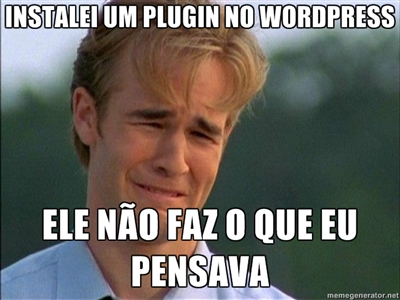
\includegraphics[height=0.8\textheight]{./img/plugins-install.jpg}
\end{center}
\end{frame}

\begin{frame}{Liberando na comunidade}
\begin{itemize}
  \pause \item Requerer hospedagem no repositório SVN oficial
  \pause \item Escrever a documentação
  \pause \item Fazer uma imagem de apresentação
  \pause \item Avaliar requisições de suporte e gerenciar traduções
\end{itemize}
\end{frame}

\begin{frame}{\texttt{readme.txt} de um plugin}
  \lstinputlisting{./code/plugin-readme.txt}
\end{frame}

\begin{frame}
\begin{center}
  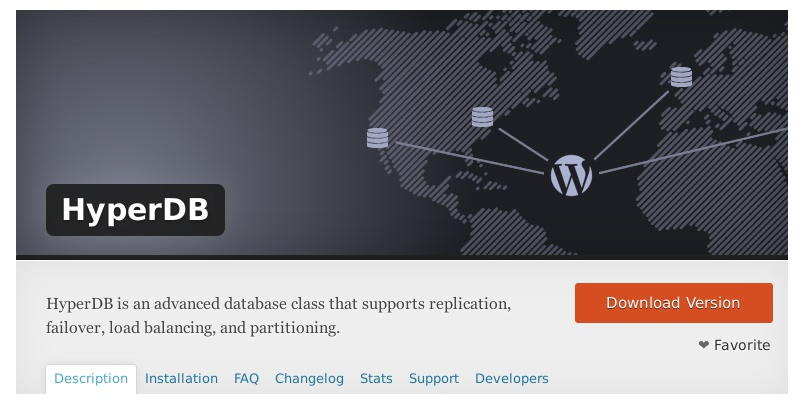
\includegraphics[width=0.95\textwidth]{./img/hyperdb-screen.jpg}
\end{center}
\end{frame}

\section{Considerações Finais}

\begin{frame}{Considerações Finais}
\begin{itemize}
  \pause \item Interfaces altamente flexíveis
  \pause \item Conjunto de ferramentas amplo e disponível
  \pause \item Fácil acesso às informações pelo desenvolvedor
  \pause \item Não tem desculpa para não codificar e suportar um
    plugin com qualidade
\end{itemize}
\end{frame}

\begin{frame}
\begin{center}
  
\includegraphics[height=0.8\textheight]{./img/thank-you.jpg}
\end{center}
\end{frame}

\begin{frame}{Referências}
\begin{itemize}
  \item Codex: Writing a Plugins \\
    \url{http://codex.wordpress.org/Writing_a_Plugin}
  \item WordPress Answers
    \url{http://wordpress.stackexchange.com/questions/715/objective-best-practices-for-plugin-development}
\end{itemize}
\end{frame}

\end{document}
